\documentclass[a4paper,twoside]{article}
\usepackage[T1]{fontenc}
\usepackage[bahasa]{babel}
\usepackage{graphicx}
\usepackage{graphics}
\usepackage{float}
\usepackage[cm]{fullpage}
\pagestyle{myheadings}
\usepackage{etoolbox}
\usepackage{setspace} 
\usepackage{comment}
\usepackage{lipsum} 
\usepackage{hyperref} 
\setlength{\headsep}{30pt}
\usepackage[inner=2cm,outer=2.5cm,top=2.5cm,bottom=2cm]{geometry} %margin
% \pagestyle{empty}

\hyphenation{di-se-dia-kan}
\hyphenation{ter-in-te-gra-si}

\makeatletter
\renewcommand{\@maketitle} {\begin{center} {\LARGE \textbf{ \textsc{\@title}} \par} \bigskip {\large \textbf{\textsc{\@author}} }\end{center} }
\renewcommand{\thispagestyle}[1]{}
\markright{\textbf{\textsc{AIF18401/AIF18402 \textemdash Rencana Kerja Skripsi \textemdash Sem. Ganjil 2021/2022}}}

\newcommand{\HRule}{\rule{\linewidth}{0.4mm}}
\renewcommand{\baselinestretch}{1}
\setlength{\parindent}{0 pt}
\setlength{\parskip}{6 pt}

\onehalfspacing
 
\begin{document}

\title{\@judultopik}
\author{\nama \textendash \@npm} 

%tulis nama dan NPM anda di sini:
\newcommand{\nama}{Christian S. G. Patrick Nasira}
\newcommand{\@npm}{2017730089}
\newcommand{\@judultopik}{Manajemen Tempat Duduk pada OXAM} % Judul/topik anda
\newcommand{\jumpemb}{1} % Jumlah pembimbing, 1 atau 2
\newcommand{\tanggal}{21/10/2021}

% Dokumen hasil template ini harus dicetak bolak-balik !!!!

\maketitle

\pagenumbering{arabic}

\section{Deskripsi}
\label{sec:deskripsi}
\begin{comment}
Tuliskan deskripsi dari topik skripsi yang akan anda ajukan. Di sini dapat dituliskan latar belakang, seperti apa penelitian yang sudah ada sebelumnya dan apa yang akan anda kerjakan. Sertakan gambar agar penjelasan anda menjadi lebih baik.

Pada skripsi ini, akan dibuat sebuah perangkat lunak yang dapat menampilkan visualisasi dan simulasi kerumunan orang yang berkunjung ke sebuah museum. Dengan menggunakan perangkat lunak tersebut, pengelola museum dapat mengatur tempat peletakan objek sehingga tidak terjadi kerumunan yang terlalu padat.

Dari berbagai macam teknik yang dapat digunakan untuk melakukan simulasi kerumunan, dipilih dua buah teknik yaitu teknik {\it flow tiles} dan {\it social force model (steering behaviour)}.

Dst, dst, dst, \ldots\ldots\ldots 

Perangkat lunak akan dibuat dengan bantuan {\it framework} OpenSteer. Sebagai studi kasus, museum yang digunakan untuk melakukan simulasi adalah Museum Geologi Bandung.

Dst, dst, dst, \ldots\ldots\ldots 
\end{comment}

\begin{comment}
OXAM merupakan aplikasi manajemen ujian di labftis.

Topik ini merupakan pengembangan skripsi dengan kode RCP4703 yang dikerjakan oleh Gunawan Christianto (2016730011).

Pada skripsi tersebut terdapat beberapa saran dan usulan pada saat sidang yang secara umum terletak pada pengaturan tempat duduk peserta ujian.
\end{comment}

Laboratorium Komputasi Fakultas Teknologi Informasi dan Sains (FTIS) merupakan fasilitas yang disediakan untuk menunjang kegiatan perkuliahan yang bersifat praktik di lingkungan FTIS UNPAR. Sebagai contoh, kegiatan yang ditunjang adalah ujian praktik di masa UTS dan UAS bagi jurusan Informatika, Matematika, dan Fisika. Pihak-pihak yang terlibat dalam kegiatan ujian praktik ini, antara lain Admin Lab yang bertugas untuk mempersiapkan ruang ujian dan membantu apabila ada kendala pada saat ujian berlangsung,  Koordinator Ujian yang bertugas untuk mengkoordinasikan jalannya ujian, Pengawas Ujian yang bertugas mengawasi jalannya ujian, serta Peserta yang akan mengikuti ujian.

\setlength\parindent{24pt}

Terdapat cukup banyak kendala teknikal pada persiapan dan pelaksanaan ujian. Sebagai contoh, ketika ujian berlangsung komputer yang sudah disediakan bermasalah, sehingga \textit{file} ujian peserta harus dipindahkan ke komputer lainnya. Hal ini dilakukan oleh Admin Lab secara manual dengan cara membuat ulang \textit{script} untuk mengatur \textit{permission} dari \textit{file} ujian yang akan digunakan di komputer baru. Kendala lainnya adalah \textit{timer} ujian di Lab yang tidak sinkron dengan \textit{database}. Hal ini dikarenakan \textit{timer} ujian di Lab dimulai secara manual oleh Pengawas Ujian dan tidak terintegrasi dengan database. Guna menangani kendala-kendala ini dibuatlah sebuah aplikasi yang bernama OXAM. 

OXAM merupakan sebuah aplikasi manajemen ujian di Laboratorium Komputasi FTIS atau Lab.~FTIS yang dirancang untuk mempermudah Admin, Koordinator Ujian dan Pengawas untuk mempersiapkan hal-hal yang bersifat administratif terkait dengan ujian. Beberapa contoh kegiatan administratif yang kini sudah dapat ditangani menggunakan OXAM adalah: (1) pemilihan posisi duduk peserta ujian oleh Admin secara interaktif disertai pembuatan daftar hadir peserta ujian dan \textit{script} penyebaran bahan ujian; (2) sinkronisasi waktu ujian, penambahan, maupun pengubahan waktu ujian melalui OXAM; (3) pemindahan posisi ujian peserta; (4)~fitur notifikasi hal-hal terkait ujian melalui OXAM; (5) pengarsipan hasil ujian  hingga pengiriman hasil ujian kepada dosen matakuliah yang dilakukan melalui OXAM.

Pada saat topik ini dikeluarkan, OXAM telah dikembangkan hingga versi yang kelima. Topik~ini (RCP5103) merupakan topik lanjutan dari topik dengan kode RCP4703 yang dikerjakan oleh Gunawan Christianto (2016730011). Pengerjaan dari topik dengan kode RCP4703 telah menghasilkan sebuah sistem yang lebih baik dari versi sebelumnya. Hal ini dapat dilihat dengan adanya tampilan UI OXAM yang lebih interaktif dan tambahan fitur-fitur yang sudah disebutkan sebelumnya. Terdapat beberapa saran dan masukan yang diberikan pada saat sidang untuk topik dengan kode RCP4703. Beberapa saran dan masukan tersebut secara umum terletak pada pengaturan tempat duduk peserta ujian.

\begin{figure}
    \centering
    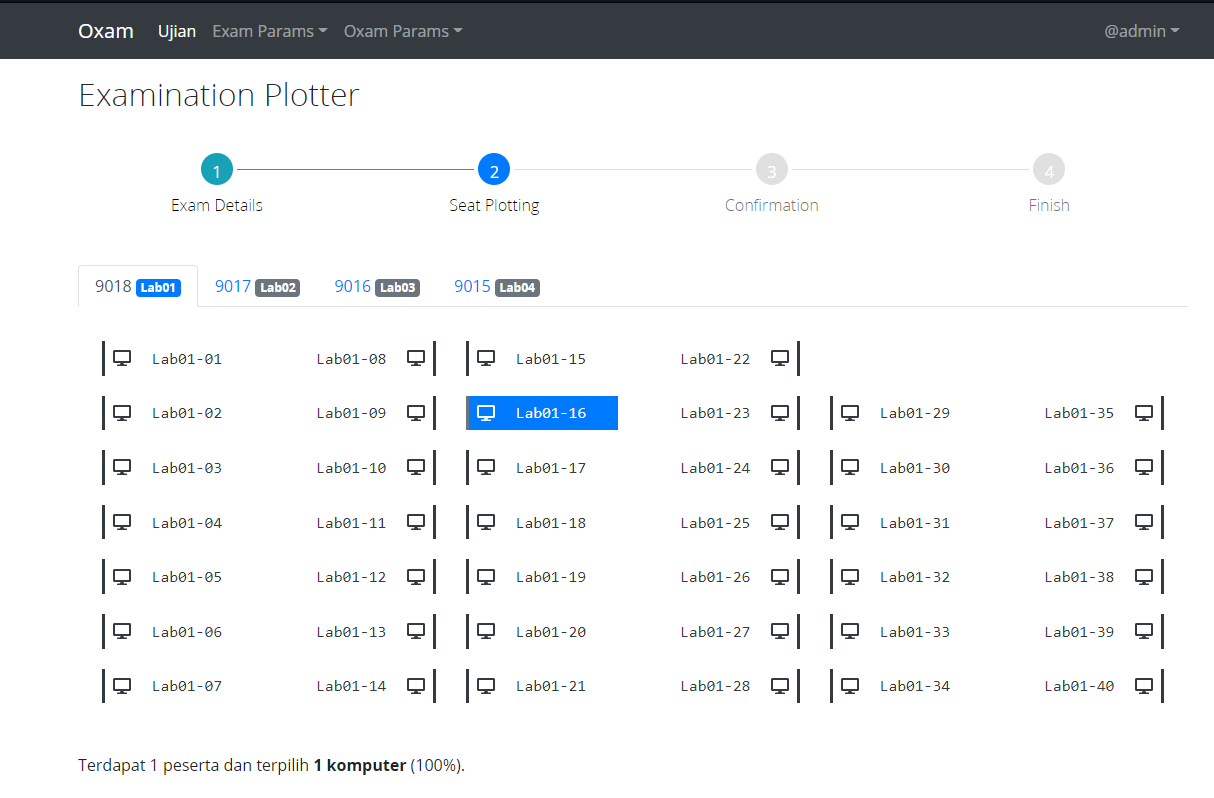
\includegraphics[width=0.8\textwidth]{images/seat-plotting.PNG}
    \caption{Pemilihan posisi duduk peserta ujian yang dilakukan secara manual.}
    \label{fig:seat-plotting}
\end{figure}

Gambar \ref{fig:seat-plotting} merupakan tampilan pada OXAM ketika Admin melakukan pemilihan posisi ujian peserta. Pemilihan posisi ujian dilakukan secara manual dengan cara memilih satu per satu komputer yang akan digunakan. Komputer-komputer yang sudah dipilih kemudian digunakan untuk menempatkan peserta ujian secara acak. OXAM kemudian akan menghasilkan \textit{script} berdasarkan hasil pemilihan acak yang nantinya akan dijalankan di \textit{server} untuk mendistribusikan berkas ujian. 

Berdasarkan ilustrasi di atas, terdapat beberapa usulan pengembangan pada mekanisme pemilihan posisi ujian. Usulan berfokus pada pencegahan terjadinya \textit{human error} pada saat pemilihan komputer yang dilakukan satu per satu, padahal sebenarnya dapat diotomatisasi berdasarkan jumlah peserta ujian. Selain itu, tampilan pada saat akan memilih posisi tidak menggambarkan kondisi komputer secara \textit{real time}. Pencatatan kondisi komputer dilakukan secara manual dan terpisah dari sistem. Hal ini mengakibatkan komputer yang dipilih mungkin saja berada dalam kondisi rusak, kosong tidak tersedia, memiliki masalah jaringan, atau masalah teknikal lainnya yang dapat mengakibatkan kendala pada saat pelaksanaan ujian. Dengan adanya pemeriksaan kondisi komputer secara \textit{real time} yang terintegrasi dengan sistem, masalah-masalah tersebut dapat terdeteksi lebih awal. Pemilihan secara acak pun dapat disesuaikan dengan ketersediaan komputer yang ada.

Usulan lainnya terkait dengan posisi komputer dan juga \textit{layout} tiap ruang lab ujian yang dibuat secara \textit{hardcode}. Jika terjadi perpindahan ruang lab yang mengakibatkan berubahnya layout ruangan, maka aplikasi menjadi tidak dapat digunakan. Pengembangan diharapkan dapat mempermudah penambahan atau pergantian \textit{layout} pada aplikasi OXAM yang dilakukan secara interaktif.

Selain usulan terkait pemilihan posisi dan \textit{layout} ruangan lab, terdapat pula usulan untuk menambahkan mode berbasis token. Dengan adanya mode berbasis token, \textit{login} dapat dilakukan tanpa bergantung pada IP \textit{address} komputer serta peserta dapat duduk dimana saja. Dengan adanya mode berbasis token kegunaan OXAM dapat bertambah selain untuk UTS dan UAS, yakni digunakan untuk praktikum, kuis, ataupun latihan. 

Berdasarkan usulan tersebut, maka pada skripsi ini akan dilakukan pengembangan pada OXAM dengan lebih berfokus pada pengembangan mekanisme pemilihan posisi ujian, pengaturan \textit{layout} yang dibuat agar lebih interaktif, dan penambahan mode berbasis token. 

\vspace{-0.1cm}
\section{Rumusan Masalah}
\label{sec:rumusan}
%Tuliskan rumusan dari masalah yang akan anda bahas pada skripsi ini. Rumusan masalah biasanya berupa kalimat pertanyaan. Gunakan itemize seperti contoh di bagian Deskripsi Perangkat Lunak.
Berdasarkan deksripsi yang sudah dipaparkan di bagian \ref{sec:deskripsi}, terdapat beberapa hal yang menjadi poin utama untuk dijadikan sebagai rumusan masalah pada skripsi ini. Beberapa hal tersebut adalah:
\begin{enumerate}
    \item Bagaimana mekanisme yang diperlukan untuk menangani manajemen ruang pada laboratorium komputasi FTIS secara interaktif dan penempatan posisi peserta ujian dengan tetap memperhatikan keadaan komputer secara \textit{real time}?
    \item Bagaimana mekanisme yang diperlukan untuk menerapkan mode berbasis token dalam penggunaan OXAM?
    \item Bagaimana implementasi mode berbasis token pada OXAM?
    \item Bagaimana implementasi untuk menghasilkan sistem manajemen ruang pada laboratorium komputasi FTIS secara interaktif dan pemilihan penempatan posisi peserta ujian yang memperhatikan keadaan komputer secara \textit{real time}?
\end{enumerate}

\section{Tujuan}
%Tuliskan tujuan dari topik skripsi yang anda ajukan. Tujuan penelitian biasanya berkaitan erat dengan pertanyaan yang diajukan di bagian rumusan masalah. Gunakan itemize seperti contoh di bagian Deskripsi Perangkat Lunak.

Berdasarkan bagian \ref{sec:deskripsi} dan bagian \ref{sec:rumusan}, dapat ditetapkan beberapa hal yang menjadi tujuan dari skripsi ini.

\begin{enumerate}
    %\item Mengetahui mekanisme penanganan manajemen ruang pada laboratorium komputasi FTIS secara interaktif dan pemilihan posisi peserta ujian dengan memperhatikan keadaan atau kondisi \textit{real time} dari komputer
    \item Spesifikasi kebutuhan dan rancangan untuk membuat sistem penanganan manajemen ruang pada laboratorium komputasi FTIS secara interaktif dan pemilihan posisi peserta ujian dengan memperhatikan keadaan atau kondisi \textit{real time} dari komputer
    \item Spesifikasi kebutuhan  dan rancangan untuk menerapkan mode berbasi token pada OXAM
    \item Sistem manajemen ruang laboratorium komputasi FTIS secara interaktif menggunakan \textit{canvas} dan sistem pemilihan posisi ujian peserta secara acak dengan memperhatikan keadaan atau kondisi \textit{real time} dari komputer yang terintegrasi dengan OXAM
    %\item Mengetahui mekanisme yang diperlukan untuk menerapkan mode berbasis token dalam penggunaan OXAM
    %\item Implementasi sistem manajemen ruang pada laboratorium komputasi FTIS yang interaktif dan pemilihan penempatan posisi peserta ujian yang memperhatikan keadaan komputer secara \textit{real time}
    %\item Implementasi sistem manajemen ruang pada laboratorium komputasi FTIS secara interaktif dan pemilihan penempatan posisi peserta ujian dengan memperhatikan keadaan komputer secara \textit{real time}
    %\item Implementasi mode berbasis token pada OXAM
    \item Mode berbasis token pada OXAM yang dapat berjalan tanpa menggangu mode berbasi IP \textit{Address}
\end{enumerate}

\section{Deskripsi Perangkat Lunak}
%Tuliskan deksripsi dari perangkat lunak yang akan anda hasilkan. Apa saja fitur yang disediakan oleh PL tersebut dan apa saja kemampuan dari PL tersebut. Perhatikan contoh di bawah ini:

Perangkat lunak akhir yang akan dibuat memiliki fitur minimal sebagai berikut:
\begin{itemize}
	
	\item Pengguna dengan \textit{role} Admin dapat menambahkan, melakukan modifikasi, menyimpan hasil pengaturan \textit{layout}, serta menghapus \textit{layout} ruang laboratorium secara interaktif
	\item Program dapat menampilkan kondisi komputer pada ruangan laboratorium secara \textit{real time} pada saat akan dilakukan pemilihan posisi ujian oleh pengguna dengan \textit{role} Admin
	\item Program dapat melakukan pengacakan posisi ujian di lab berdasarkan \textit{list} peserta yang diberikan dengan tetap memperhatikan kondisi komputer di ruang lab
    \item Pengguna dalam hal ini peserta ujian, Koordinator, dan Admin dapat melakukan login dari luar ruang laboratorium
	\item Pengguna dengan \textit{role} Admin atau Koordinator Ujian dapat membuat ujian tanpa harus melakukan pemilihan posisi
    \item Distribusi bahan ujian dapat dilakukan tanpa menggunakan \textit{script} (bahan ujian disediakan untuk diunduh secara \textit{online})
	\item Pengguna dalam hal ini peserta ujian dapat mengikuti ujian tanpa harus berada di lab komputer
	\item Pengguna dalam hal ini peserta ujian dapat mengunduh bahan ujian yang disediakan untuk ujian yang menggunakan mode berbasis token
	
		
\end{itemize}

\section{Detail Pengerjaan Skripsi}
Berdasarkan deskripsi dan tujuan yang dipaparkan di atas, bagian-bagian yang menjadi pekerjaan pada skripsi ini adalah sebagai berikut :
	\begin{enumerate}
	\item Mempelajari cara kerja OXAM dan skripsi dari Christian Toqiang (2016730011)
	\item Mempelajari ReactJS sebagai \textit{library front-end}
	\item Mempelajari FatFree  sebagai \textit{framework} yang digunakan untuk \textit{back-end}
	\item Mengumpulkan kebutuhan dan melakukan analisis dampak
	\item Merancang dan mengimplementasi perangkat lunak
	\item Melakukan pengujian perangkat lunak
	\item Melaporkan hasil penelitian dalam bentuk dokumen skripsi
	\end{enumerate}

\section{Rencana Kerja}
Rincian capaian yang direncanakan di Skripsi 1 adalah sebagai berikut:
\begin{enumerate}
\item Mempelajari cara kerja OXAM dan skripsi dari Gunawan Christianto (2016730011)
\item Mempelajari ReactJS sebagai \textit{library front-end}
\item Mempelajari FatFree  sebagai \textit{framework} yang digunakan untuk \textit{back-end}
\item Mengumpulkan kebutuhan dan melakukan analisis dampak
\end{enumerate}

Sedangkan yang akan diselesaikan di Skripsi 2 adalah sebagai berikut:
\begin{enumerate}

\item Merancang dan mengimplementasi perangkat lunak
\item Melakukan pengujian perangkat lunak
\item Melaporkan hasil penelitian dalam bentuk dokumen skripsi
\end{enumerate}

\vspace{1cm}
\centering Bandung, \tanggal\\
\begin{comment}
\begin{figure}[H]
    \centering
    \includegraphics[width=0.15\textwidth]{images/tdt-small.png}
    \label{fig:tdt-mahasiswa}
\end{figure}
\end{comment}
 \vspace{2cm}\nama \\ 
\vspace{1cm}

Menyetujui, \\
\ifdefstring{\jumpemb}{2}{
\vspace{1.5cm}
\begin{centering} Menyetujui,\\ \end{centering} \vspace{0.75cm}
\begin{minipage}[b]{0.45\linewidth}
% \centering Bandung, \makebox[0.5cm]{\hrulefill}/\makebox[0.5cm]{\hrulefill}/2013 \\
\vspace{2cm} Nama: \makebox[3cm]{\hrulefill}\\ Pembimbing Utama
\end{minipage} \hspace{0.5cm}
\begin{minipage}[b]{0.45\linewidth}
% \centering Bandung, \makebox[0.5cm]{\hrulefill}/\makebox[0.5cm]{\hrulefill}/2013\\
\vspace{2cm} Nama: \makebox[3cm]{\hrulefill}\\ Pembimbing Pendamping
\end{minipage}
\vspace{0.5cm}
}{
% \centering Bandung, \makebox[0.5cm]{\hrulefill}/\makebox[0.5cm]{\hrulefill}/2013\\
%\vspace{2cm} Nama: \makebox[3cm]{\hrulefill}\\ Pembimbing Tunggal
\vspace{2cm}Raymond Chandra Putra, S.T., M.T.\\ Pembimbing Tunggal
}
\end{document}

